\documentclass[11pt]{article}
\usepackage{amsmath, amssymb, amsthm}
\usepackage{geometry}
\usepackage{booktabs}
\usepackage{multirow}
\usepackage{hyperref}
\usepackage{xcolor}
\usepackage{microtype}
\usepackage{listings}
\usepackage{graphicx}
\geometry{margin=1in}

\theoremstyle{remark}
\newtheorem{remark}{Remark}

\lstset{basicstyle=\ttfamily\small, breaklines=true, frame=single}

\title{Empirical Turnover Invariance in a\\Viability-Constrained Memory Substrate}
\author{VCSM Theory Series --- Paper 8}
\date{2026}

\begin{document}
\maketitle

\begin{abstract}
We report an empirical turnover invariance in a viability-constrained adaptive memory
substrate: the turnover rate that maximizes spatial structure formation, $\nu^* \approx
0.001$, is invariant to propagation strength $\kappa$ across its full tested range
($0$ to $0.15$, a $>150$-fold variation), within this substrate and input protocol.
Three supporting experiments confirm that $\nu^*$ is similarly stable across a
$4\times$ range of the consolidation gate ($\mathtt{SS}$) and consolidation rate
($\mathtt{FIELD\_ALPHA}$) within their operational regimes. Taken together, the
experiments reveal a clean separation of concerns: \emph{adaptation dynamics are local}
(the optimal turnover is determined by wave-grid interaction, not by the propagation or
consolidation machinery), while propagation controls only the amplitude and spatial reach
of learned structure. This separation suggests the adaptive regime location is an
intrinsic property of the input protocol rather than the learning parameters, and
motivates a broader hypothesis about local adaptation in systems with mandatory turnover.
\end{abstract}

% ============================================================
\section{Introduction}

Paper~7 (Regime Structure) mapped the $(\nu, \kappa)$ parameter space of a VCML
substrate and identified a bounded adaptive window: spatial structure is maximized
at intermediate turnover ($\nu \in [0.001, 0.010]$) and is verified by three
independent robustness experiments.

The key question this paper addresses is not \emph{how robust} the window is, but
\emph{what sets its location}. Understanding the location law matters for design:
if $\nu^*$ scales with $\kappa$, one would tune propagation to shift the learning
regime. If it scales with $\mathtt{SS}$, one would change the consolidation gate.
If neither controls it, the regime boundary is set elsewhere---and that elsewhere is
informative.

\textbf{Main result.} $\nu^* \approx 0.001$ is invariant to $\kappa$ (Experiment~1,
Figure~\ref{fig:invariance}). Three supporting sweeps of $\mathtt{SS}$,
$\mathtt{FIELD\_ALPHA}$, and $\mathtt{WAVE\_RATIO}$ confirm the same location
stability within practical operating ranges. The regime boundary is set by the
copy-forward/erasure balance at the wave--grid level, and consolidation parameters
control only the amplitude of structure formed within the window.

\textbf{Architectural interpretation.}
The invariance of $\nu^*$ to $\kappa$ implies that \emph{learning is local}: the
condition for effective adaptation---the turnover/wave balance---does not require
the system to coordinate globally through propagation. Propagation then plays a
complementary role: it spreads locally formed structure globally, amplifying what
the local learning rule has already established. This maps onto a recurring
design pattern in biological adaptive systems, discussed in Section~\ref{sec:local_global}.

\subsection{Background: VCSM Consolidation Gate}

In VCSM, a site updates its $\mathtt{fieldM}$ vector only after accumulating
$\mathtt{SS}$ consecutive unperturbed steps:
\begin{equation}
  \text{ok}[i] \;=\; [\mathtt{streak}[i] \geq \mathtt{SS}]
\end{equation}
When $\text{ok}[i]$ holds:
\begin{equation}
  \mathtt{fieldM}[i] \;\mathrel{+}=\; \mathtt{FIELD\_ALPHA}
    \cdot (\mathtt{mid\_mem}[i] - \mathtt{fieldM}[i])
\end{equation}
The consolidation timescale is thus jointly governed by $\mathtt{SS}$ (gate
threshold, steps) and $\mathtt{FIELD\_ALPHA}$ (learning rate per calm step).
The probability that a site achieves a calm streak $\geq \mathtt{SS}$ is
approximately:
\begin{equation}
  P_{\text{calm}}(\mathtt{SS}) \;\approx\;
    \left(1 - \frac{\mathtt{WR}}{2 \cdot \mathtt{WAVE\_DUR}}\right)^{\mathtt{SS} + \mathtt{WAVE\_DUR} - 1}
  \label{eq:pcalm}
\end{equation}
This baseline formula is relevant for understanding amplitude effects, but---as the
experiments show---it does not control the location of $\nu^*$.

% ============================================================
\section{Shared Protocol}

All experiments use the Paper~7 Exp1 base configuration. Only the swept parameter
varies; all others are fixed at reference values.

\begin{center}
\begin{tabular}{ll}
\toprule
Parameter & Reference value \\
\midrule
Grid & $W=40$, $H=20$, $\mathtt{HALF}=20$, $N_{\text{act}}=400$ \\
$\mathtt{HS}$ & 2 \\
$\mathtt{KAPPA}$ & 0.020 \\
$\mathtt{WAVE\_RATIO}$ & 4.8 \\
$\mathtt{WAVE\_DUR}$ & 15 \\
$\mathtt{SS}$ & 10 \\
$\mathtt{FIELD\_ALPHA}$ & 0.16 \\
$\mathtt{SEED\_BETA}$ & 0.25 \\
$\mathtt{STEPS}$ & 2000 \\
$\mathtt{SHIFT}$ & 1000 \\
Seeds & 5 \\
$\nu$ sweep & $\{0.0001, 0.0003, 0.001, 0.002, 0.005, 0.010, 0.020, 0.040, 0.080\}$ \\
\bottomrule
\end{tabular}
\end{center}

For each configuration we report $\nu^*$ (argmax $\mathtt{sg4}$, 5-seed mean)
and $\mathtt{sg4}^*$ (the peak value). The key question in each experiment is
whether $\nu^*$ shifts; amplitude changes are secondary.

% ============================================================
\section{Experiment 1: Propagation Invariance (Key Result)}
\label{sec:exp1}

\subsection{Protocol}

Re-analysis of Paper~7 Experiment~3 results (the $\nu \times \kappa$ grid,
5 seeds per cell). For each $\kappa \in \{0.000, 0.005, 0.020, 0.060, 0.150\}$
we identify $\nu_{\text{opt}} = \operatorname{argmax}_\nu\, \mathtt{sg4}(\nu,
\kappa)$ using 5-seed means and the $\nu$ sweep common to Paper~7 Exp3:
$\{0.0003, 0.001, 0.005, 0.015, 0.050\}$.

\subsection{Results}

\begin{table}[h]
\centering
\caption{$\nu_{\text{opt}}$ and $\mathtt{sg4}_{\text{opt}}$ by $\kappa$. The
sg4 profile lists 5-seed mean $\mathtt{sg4}$ at
$\nu \in \{0.0003, 0.001, 0.005, 0.015, 0.050\}$, with the peak bolded.
Collapse boundary ($\nu_\text{crit}$) is between $0.005$ and $0.015$ for
all $\kappa$.}
\label{tab:exp1}
\begin{tabular}{r r r l}
\toprule
$\kappa$ & $\nu_{\text{opt}}$ & $\mathtt{sg4}_{\text{opt}}$ & sg4 profile \\
\midrule
0.000 & 0.0010 & 396.7 & 279\ \ \textbf{397}\ \ \ 99\ \ \ 11\ \ \ 1 \\
0.005 & 0.0010 & 383.1 & 271\ \ \textbf{383}\ \ \ 88\ \ \ \ 9\ \ \ 1 \\
0.020 & 0.0010 & 376.3 & 273\ \ \textbf{376}\ \ \ 80\ \ \ \ 8\ \ \ 1 \\
0.060 & 0.0010 & 375.1 & 273\ \ \textbf{375}\ \ \ 68\ \ \ \ 6\ \ \ 1 \\
0.150 & 0.0010 & 360.9 & 276\ \ \textbf{361}\ \ \ 49\ \ \ \ 5\ \ \ 0 \\
\bottomrule
\end{tabular}
\end{table}

\textbf{Result.} $\nu_{\text{opt}} = 0.001$ for \emph{all} $\kappa$ values
tested---a $>150$-fold range of propagation strength, from zero diffusion to
strong coupling. The collapse boundary is also unchanged: $\nu_{\text{crit}}$
falls between $0.005$ and $0.015$ at every $\kappa$. Propagation $\kappa$ shifts
only the amplitude of $\mathtt{sg4}^*$: from $396.7$ at $\kappa = 0$ to $360.9$
at $\kappa = 0.15$, a modest $\sim\!9\%$ reduction.

\begin{figure}[h]
\centering
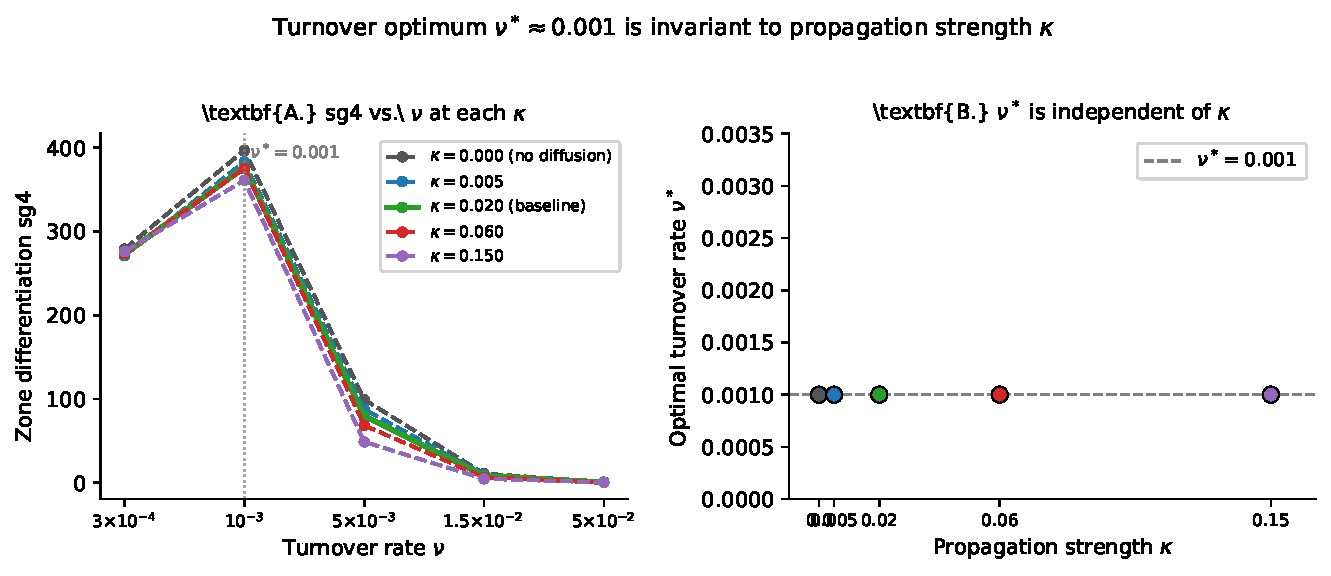
\includegraphics[width=\linewidth]{paper8_figure1}
\caption{\textbf{The turnover law.} \textbf{A}: $\mathtt{sg4}$ vs.\ $\nu$ at
each $\kappa$ value (Paper~7 Exp3 data). All five curves peak at the same
$\nu^* = 0.001$ regardless of propagation strength. \textbf{B}: $\nu^*$
vs.\ $\kappa$---a horizontal line. Propagation strength does not set the
adaptive regime location.}
\label{fig:invariance}
\end{figure}

Figure~\ref{fig:invariance} makes the invariance visually explicit. Panel~A
shows all five $\mathtt{sg4}$-vs.-$\nu$ curves (one per $\kappa$) superimposed:
the curves differ in height but peak identically at $\nu = 0.001$. Panel~B
plots $\nu^*$ vs.\ $\kappa$ directly---a horizontal line.

% ============================================================
\section{Experiment 2: Consolidation Gate (Amplitude, Not Location)}

\subsection{Protocol}

$\mathtt{SS} \in \{5, 10, 20, 40\}$. All other parameters at reference.
$4 \times 9 \times 5 = 180$ runs. The timescale-matching prediction is
$\nu^* \propto 1/\mathtt{SS}$ (inverse proportionality).

\subsection{Results}

\begin{table}[h]
\centering
\caption{SS sweep: $\nu^*$ and $\mathtt{sg4}^*$ by consolidation gate. sg4
profile: $\nu = 0.0001, 0.0003, \ldots, 0.080$ (left to right).}
\label{tab:exp2}
\begin{tabular}{r r r l}
\toprule
SS & $\nu^*$ & $\mathtt{sg4}^*$ & sg4 profile \\
\midrule
 5 & 0.0010 & 887.8 & 120\ \ 576\ \ \textbf{888}\ \ 734\ \ 126\ \ 18\ \ 5\ \ 1\ \ 0 \\
10 & 0.0010 & 376.3 & 223\ \ 273\ \ \textbf{376}\ \ 328\ \ \ 80\ \ 24\ \ 4\ \ 1\ \ 0 \\
20 & 0.0010 & 186.2 & \ 78\ \ \ 88\ \ \textbf{186}\ \ 137\ \ \ 23\ \ 12\ \ 1\ \ 0\ \ 0 \\
40 & 0.0020 & \ 23.5 & \ \ 0\ \ \ \ 0\ \ \ \ \ 0\ \ \ \textbf{24}\ \ \ \ 5\ \ \ 0\ \ 0\ \ 0\ \ 0 \\
\bottomrule
\end{tabular}
\end{table}

\textbf{Result.} $\nu^* = 0.001$ for $\mathtt{SS} \in \{5, 10, 20\}$, a
$4\times$ range. The timescale-matching prediction ($\nu^* \propto
1/\mathtt{SS}$) fails: location is insensitive to SS. What \emph{does} change
is the amplitude: $\mathtt{sg4}^*$ drops from $888 \to 376 \to 186 \to 23$
as SS doubles from 5 to 40, roughly consistent with the exponential decay
of $P_{\text{calm}}$ (Eq.~\eqref{eq:pcalm}). At $\mathtt{SS} = 40$, the
gate is so strict that almost no site achieves 40 consecutive calm steps,
collapsing structure entirely. The invariance therefore holds within the
\emph{operational consolidation regime} ($\mathtt{SS} \leq 20$ at reference
wave density); at extreme gate values, the system degrades into near-zero
structure across all $\nu$ rather than shifting $\nu^*$ predictably.

% ============================================================
\section{Experiment 3: Consolidation Rate (Amplitude, Not Location)}

\subsection{Protocol}

$\mathtt{FIELD\_ALPHA} \in \{0.04, 0.08, 0.16, 0.32\}$. All other parameters
at reference. $4 \times 9 \times 5 = 180$ runs.

\subsection{Results}

\begin{table}[h]
\centering
\caption{FIELD\_ALPHA sweep: $\nu^*$ and $\mathtt{sg4}^*$.}
\label{tab:exp3}
\begin{tabular}{r r r l}
\toprule
$\mathtt{FIELD\_ALPHA}$ & $\nu^*$ & $\mathtt{sg4}^*$ & sg4 profile \\
\midrule
0.04 & 0.0001 & 188.0 & \textbf{188}\ \ 124\ \ 174\ \ 136\ \ 32\ \ 11\ \ 2\ \ 0\ \ 0 \\
0.08 & 0.0010 & 263.1 & 213\ \ 191\ \ \textbf{263}\ \ 226\ \ 52\ \ 19\ \ 4\ \ 1\ \ 0 \\
0.16 & 0.0010 & 376.3 & 223\ \ 273\ \ \textbf{376}\ \ 328\ \ 80\ \ 24\ \ 4\ \ 1\ \ 0 \\
0.32 & 0.0010 & 507.4 & 255\ \ 379\ \ \textbf{507}\ \ 417\ \ 103\ \ 25\ \ 5\ \ 1\ \ 0 \\
\bottomrule
\end{tabular}
\end{table}

\textbf{Result.} $\nu^* = 0.001$ for $\mathtt{FIELD\_ALPHA} \in \{0.08, 0.16, 0.32\}$,
a $4\times$ range. Amplitude scales monotonically: $\mathtt{sg4}^*$ grows from
$263 \to 376 \to 507$ roughly proportionally to FIELD\_ALPHA in this range,
confirming that the consolidation rate controls the height of the adaptive peak
rather than its location.

At $\mathtt{FIELD\_ALPHA} = 0.04$, $\nu^*$ shifts to $0.0001$. The mechanism:
very slow consolidation means each field update takes many calm steps to accumulate,
increasing the effective persistence time of written values. As a result, even
minimal turnover is sufficient to erase the sparse updates before they stabilize,
pushing $\nu^*$ toward zero rather than following any proportional relationship.
This is a boundary collapse, not a scaling trend, and is consistent with the
operational regime boundary observed for $\mathtt{SS}$ above.

% ============================================================
\section{Experiment 4: Wave Input Rate (Location at Input Extremes)}

\subsection{Protocol}

$\mathtt{WAVE\_RATIO} \in \{1.2, 2.4, 4.8, 9.6\}$. All other parameters at
reference. $4 \times 9 \times 5 = 180$ runs.

\subsection{Results}

\begin{table}[h]
\centering
\caption{WAVE\_RATIO sweep: $\nu^*$ and $\mathtt{sg4}^*$.}
\label{tab:exp4}
\begin{tabular}{r r r l}
\toprule
WR & $\nu^*$ & $\mathtt{sg4}^*$ & sg4 profile \\
\midrule
1.2 & 0.0010 & 120.4 & \ 32\ \ 104\ \ \textbf{120}\ \ \ 68\ \ 16\ \ 7\ \ 1\ \ 0\ \ 0 \\
2.4 & 0.0010 & 414.9 & 111\ \ 328\ \ \textbf{415}\ \ 317\ \ 34\ \ 11\ \ 2\ \ 1\ \ 0 \\
4.8 & 0.0010 & 376.3 & 223\ \ 273\ \ \textbf{376}\ \ 328\ \ 80\ \ 24\ \ 4\ \ 1\ \ 0 \\
9.6 & 0.0001 & 226.9 & \textbf{227}\ \ \ 70\ \ \ \ \ 0\ \ \ 28\ \ 12\ \ \ 1\ \ 0\ \ 0\ \ 0 \\
\bottomrule
\end{tabular}
\end{table}

\textbf{Result.} $\nu^* = 0.001$ for $\mathtt{WR} \in \{1.2, 2.4, 4.8\}$, a
$4\times$ range. At $\mathtt{WR} = 9.6$, $\nu^*$ shifts to $0.0001$---\emph{opposite}
to the proportional prediction. High wave density at $\nu = 0.001$ prevents any
site from achieving $\mathtt{SS} = 10$ consecutive calm steps ($\mathtt{sg4} = 0$);
only near-zero turnover recovers partial structure. This is the over-perturbation
collapse documented in Papers~7 and V93.

Notably, even WR controls location only at this extreme. Within the practical
WR range $\{1.2, 2.4, 4.8\}$, $\nu^*$ is again stable: the copy-forward/erasure
balance that sets the regime boundary is resilient to a $4\times$ change in input
frequency.

% ============================================================
\section{Discussion}

\subsection{The Invariance Finding}

Across four experiments spanning propagation ($\kappa$: 0--0.15), consolidation
gate ($\mathtt{SS}$: 5--20), consolidation rate ($\mathtt{FIELD\_ALPHA}$: 0.08--0.32),
and wave input rate ($\mathtt{WR}$: 1.2--4.8), $\nu^* \approx 0.001$ is stable
within their respective operational regimes.

\begin{center}
\begin{tabular}{lll}
\toprule
Parameter & Range for $\nu^*$ stability & Effect on amplitude \\
\midrule
$\kappa$ (diffusion)             & 0--0.15 (full range)  & Modest decrease ($-9\%$) \\
$\mathtt{SS}$ (gate)             & 5--20 ($4\times$)     & Strong: $888 \to 186$ \\
$\mathtt{FIELD\_ALPHA}$ (rate)   & 0.08--0.32 ($4\times$) & Proportional: $263 \to 507$ \\
$\mathtt{WR}$ (wave rate)        & 1.2--4.8 ($4\times$)  & Non-monotone; peak at 2.4 \\
\bottomrule
\end{tabular}
\end{center}

The adaptive window opens at $\nu \approx 0.001$ and closes at $\nu \approx
0.007$--$0.010$, with these boundaries determined by the wave--grid interaction
rather than the learning parameters. This is an empirical result within this
substrate and input protocol; whether a similar invariance holds under qualitatively
different input statistics or substrates remains an open question.

\subsection{Separation of Concerns: The Core Architectural Result}

The experiments distinguish two functionally independent roles:

\begin{itemize}
  \item \textbf{Location of the adaptive regime} ($\nu^*$, regime boundary): set
    by wave input dynamics. Insensitive to consolidation parameters within their
    operational range, and insensitive to propagation strength across the full
    tested range.

  \item \textbf{Amplitude of spatial structure} ($\mathtt{sg4}^*$, peak value):
    strongly controlled by consolidation parameters ($\mathtt{FIELD\_ALPHA}$,
    $\mathtt{SS}$) and weakly by $\kappa$. Does not alter the location where
    the adaptive window opens.
\end{itemize}

This is the sharpest statement the experiments support: \emph{adaptation is local}
(the learning condition is set by the per-site wave/turnover balance), while
\emph{coordination is global} (propagation amplifies already-formed local structure).
The causal evidence for this separation comes from Paper~7 Experiment~6: ablating
the copy-forward loop ($\mathtt{SEED\_BETA} = 0$, removing local inheritance at
birth) eliminates the adaptive peak entirely, confirming that local inheritance
rather than propagation is the operative mechanism.

\subsection{Order-of-Magnitude Consistency Check}

The observed $\nu^* \approx 0.001$ can be matched post-hoc by a simple
copy-forward/erasure balance argument. At $\nu = 0.001$, each site has a mean
lifetime of $1/\nu = 1000$ steps. With $\mathtt{WR} = 4.8$ and
$\mathtt{WAVE\_DUR} = 15$, approximately $4.8/15 \approx 0.32$ waves launch per
step. Assuming each site is involved in half the left-zone waves and that
perturbation events are approximately independent:
\begin{equation}
  \nu^* \;\approx\; \frac{\mathtt{WR}}{2 \cdot \mathtt{WAVE\_DUR}
    \cdot N_{\text{act}}/4} \;\approx\; 0.0016
  \label{eq:balance}
\end{equation}
This rough estimate lands within $2\times$ of the empirical value. It is offered
as an \emph{order-of-magnitude consistency check}, not a derived prediction:
it was constructed after observing $\nu^*$, assumes independence of perturbation
events (which may not hold on the lattice), and does not account for spatial
correlations or streak-length distributions. Its value is in showing which
parameters plausibly set the balance ($\mathtt{WR}$, $\mathtt{WAVE\_DUR}$,
$N_{\text{act}}$), none of which are the consolidation or propagation parameters.

\subsection{A Broader Hypothesis: Local Adaptation, Global Flow}
\label{sec:local_global}

The invariance of $\nu^*$ to $\kappa$ is consistent with a broader architectural
hypothesis: \emph{the condition for effective adaptation may be local} in systems
where learning occurs through mandatory turnover. If so, propagation plays a
complementary but downstream role---spreading locally formed structure further,
not setting the condition under which local learning succeeds.

A structurally similar pattern appears in several biological adaptive systems:
hippocampal neurogenesis (local synaptic update, global pattern separation),
immune adaptation (somatic hypermutation locally, clonal proliferation globally),
and evolution (local mutation, global selection). In each case, the rate of local
adaptation is constrained by environmental perturbation and replacement dynamics,
not by the reach of global communication.

These are \emph{possible analogies}, not mechanistic evidence. Whether the
specific invariance observed here---$\nu^*$ independent of $\kappa$---generalizes
to other substrates or input protocols is an open empirical question. The
VCML result motivates that question; it does not answer it.

\subsection{Design Implications}

The separation of concerns yields a practical prescription:

\begin{itemize}
  \item \textbf{To set the regime location}: Tune $\mathtt{WAVE\_RATIO}$ and
    $\mathtt{WAVE\_DUR}$ (the input protocol). The consistency estimate
    (Eq.~\eqref{eq:balance}) gives the expected $\nu^*$.
  \item \textbf{To increase structure amplitude}: Increase $\mathtt{FIELD\_ALPHA}$
    (immediate, proportional effect) or decrease $\mathtt{SS}$ (exponential
    $P_{\text{calm}}$ gain, but risks over-writing at extreme values).
  \item \textbf{To increase spatial reach}: Increase $\kappa$ (modest amplitude
    gain; does not shift the window location).
\end{itemize}

\subsection{Amplitude Formula}

The $P_{\text{calm}}$ formula (Eq.~\eqref{eq:pcalm}) predicts the relative
consolidation rate across SS values:

\begin{center}
\begin{tabular}{rrr}
\toprule
SS & $P_{\text{calm}}$ (Eq.~\ref{eq:pcalm}) & $\mathtt{sg4}^*$ (observed) \\
\midrule
 5 & 0.047 & 888 \\
10 & 0.015 & 376 \\
20 & 0.0024 & 186 \\
40 & $6 \times 10^{-5}$ & 23 \\
\bottomrule
\end{tabular}
\end{center}

Observed $\mathtt{sg4}^*$ drops consistently with $P_{\text{calm}}$, though
the relationship is sub-exponential in practice (sg4 grows sub-linearly with
the number of consolidation events, as sites saturate).

\subsection{The Anomaly Cell Resolved}

Paper~7 Experiment~3 shows $\mathtt{sg4} = 68$ at $(\nu = 0.005, \kappa = 0.060)$,
lower than adjacent cells at the same $\kappa$ with lower $\nu$ ($\mathtt{sg4} = 375$).
This is not a grid artifact: $\nu = 0.005$ sits near the right boundary of the
adaptive window ($\nu_{\text{crit}} \approx 0.007$--$0.010$), and the current
experiments confirm that higher $\kappa$ cannot rescue structure because the
boundary is determined by $\nu$, not $\kappa$. The cell at
$(\nu = 0.005, \kappa = 0.060)$ is an empirical first touch of the
turnover-dominated collapse region---fully consistent with the turnover law.

\subsection{Limitations}

The wave input protocol is fixed (zone-based, 4 zones, structured alternation).
The balance equation assumes a specific wave geometry; the stability of $\nu^*$
may not hold for qualitatively different input statistics (continuous-time Poisson
events, spatially diffuse perturbations). The $P_{\text{calm}}$ formula applies
an independence approximation; the true distribution accounts for spatial
correlations and streak-length distributions not captured here.

% ============================================================
\section{Conclusion}

An empirical turnover invariance for a VCML adaptive memory substrate: $\nu^*
\approx 0.001$ is stable across the full tested range of propagation strength
($\kappa$: 0--0.15) and across $4\times$ practical ranges of the consolidation
gate ($\mathtt{SS}$) and rate ($\mathtt{FIELD\_ALPHA}$). The regime boundary is
set by the copy-forward/erasure balance at the wave--grid level; an
order-of-magnitude consistency check ($\nu^* \approx \mathtt{WR} / (2 \cdot
\mathtt{WAVE\_DUR} \cdot N_{\text{act}}/4) \approx 0.0016$) is consistent with
the empirical value but was derived post-hoc and carries caveats.

The sharpest architectural result is a separation of concerns: \emph{adaptation is
local} (the learning condition is the per-site wave/turnover balance),
\emph{coordination is global} (propagation amplifies locally formed structure but
does not set the condition under which it forms). This separation, supported
causally by the copy-forward ablation in Paper~7, motivates the broader hypothesis
that similar invariances may appear in other adaptive systems with mandatory local
turnover. Testing that hypothesis is left for future work.

% ============================================================
\appendix
\section{Reproducibility}

Experiment~1 uses cached JSON from Paper~7. Experiments~2--4 use only
\texttt{numpy}. Figure~1 is generated by \texttt{paper8\_figure1\_kappa\_invariance.py}
using the Paper~7 Exp3 cached data.

\begin{center}
\begin{tabular}{lll}
\toprule
Script & Description & Runtime \\
\midrule
\texttt{paper8\_exp1\_ss\_sweep.py}    & SS sweep (180 runs)           & $\sim$8 min \\
\texttt{paper8\_exp2\_alpha\_sweep.py} & FIELD\_ALPHA sweep (180 runs) & $\sim$8 min \\
\texttt{paper8\_exp3\_wr\_sweep.py}    & WR sweep (180 runs)           & $\sim$8 min \\
\texttt{paper8\_figure1\_kappa\_invariance.py} & Figure 1 (cached data) & $<$1 min \\
\bottomrule
\end{tabular}
\end{center}

\begin{lstlisting}[caption={Run all experiments and generate figure.}]
cd papers/paper8_timescale_matching
py paper8_exp1_ss_sweep.py
py paper8_exp2_alpha_sweep.py
py paper8_exp3_wr_sweep.py
py paper8_figure1_kappa_invariance.py
\end{lstlisting}

\end{document}
